\section{Creating the Index}

The first task was to create a Lucene Index on the Cranfield Documents. The main() method parses the command-line parameters, then in preparation for instantiating IndexWriter, opens a Directory, and instantiates StandardAnalyzer and IndexWriterConfig. The Cranfield File to be indexed is imported from the command line providing the location of the document. The value INDEX\_DIRECTORY is the path of the filesystem directory where all index information should be stored.  \par 

In order to index and process all the documents I created a parser for the Cranfield file .The Cranfield file was a list of documents where each document had a Title (I.), Author (A.), Bibliography (B.) and the Context (W.). The parser would read the file in line by line. Each line would be added to a variable depending on the field. Once the parser looped back to a Title context, a new document would be created. \par 
	
Upon completion of all the documents being created, they were added to an ``IndexWriter" object and also written to a Directory. This directory was analysed applying a modified Analyzer which I created. \par

The analyser in which I created will remove stop words, stem the words and normalise the characters all to lower case. Removing the stop words were words taken from the ENGLISH\_STOP\_WORDS\_SET in the ``StopAnalyser" library. The ``PorterStemFilter" library was used to stem the words when being indexed.  \par

	\begin{figure}[ht!]
		\begin{center}
			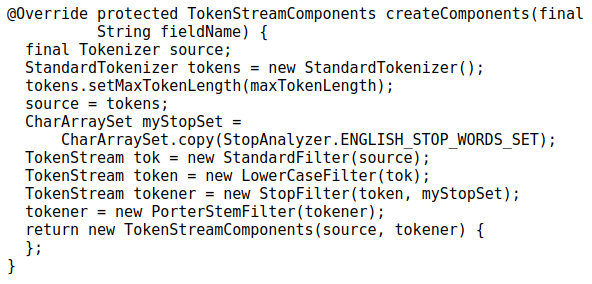
\includegraphics[scale=.4 ]{2} 
			\caption{Code Snippet of the anlayser used to stem and remove stop words}
			\label{fig:1}
		\end{center}
	\end{figure} \par

\newpage
\section{Querying the Index}
Once I created the Index I began to create a method to search the index. With the multiple fields the index contained for each document I used a ``MultiFieldParser" which searched the document for each field. The only issue was that it treats each field equally when searching in the documents.  I decided to alter weighting of importance for each field. \par

	\begin{figure}[ht!]
		\begin{center}
			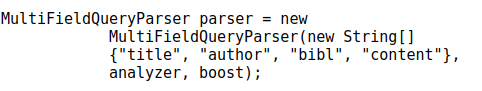
\includegraphics[scale=.5 ]{6} 
			\caption{Code Snippet of MultiFieldParser}
			\label{fig:1}
		\end{center}
	\end{figure} \par
  
In order to determine the weighting for each field, a number of tests were done to find the most accurate weightings to give the best results. From previous experience of searching for books, I would rarely use the Author or Bilbiography to search for a specfic book so I gave them a lower weighting of importance. The title and context were the main fields so they had a much higher weighting. \par

	\begin{table}[H]
		\centering
		\begin{tabular}{|p{2.5cm}|p{2.5cm}|}
			\hline
			\textbf{Context} 	& \textbf{Weighting} \\ \hline	
			Title 				& .34 \\ \hline
			Author 				& .01 \\ \hline
			Bibliography 		& .02 \\ \hline
			Context 			& .62 \\ \hline
		\end{tabular}
		\caption{Weight of each field}
		\label{table:weight}
	\end{table}

The queries were parsed from the ``cran.qry" file. They were then, just like the index file were then stemmed and removed stop words using the customised Analyser. Once all the queries were in the same format as the index file they were then put into the ``IndexSearcher" which searched the index for each query and returned all the matching documents. The max amount of results to be returned was set to 30.

	\begin{figure}[ht!]
		\begin{center}
			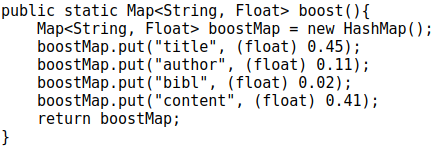
\includegraphics[scale=.4]{4} 
			\caption{Code Snippet of weighting the fields}
			\label{fig:1}
		\end{center}
	\end{figure} \par

\newpage
\section{Scoring}

The ``IndexWriterConfig" contains a method called ``setSimilarity" which sets the type of Lucene scoring that you would like to use. Similarity defines the components of Lucene scoring. From research the main four lucene scoring methods are: \par
		
	\begin{multicols}{2}
		\begin{itemize}
			\item BM25
			\item Boolean
			\item Classic
			\item lm\_dirichlet
		\end{itemize}
	\end{multicols}
	
One of the higher-level implementation such as TFIDFSimilarity (also known as Classic Similarity), which implements the vector space model with this API is one of the four I decided to use. \par 

	\begin{figure}[ht!]
		\begin{center}
			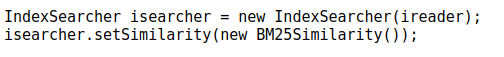
\includegraphics[scale=.5 ]{5} 
			\caption{Code Snippet of setting the Similarity when Searching}
			\label{fig:1}
		\end{center}
	\end{figure} \par

When testing it was necessary to make sure that the indexing and query searching were using the same similarity scoring as they had to be the same in order to get the right results and scores. \par
 
	\begin{figure}[ht!]
		\begin{center}
			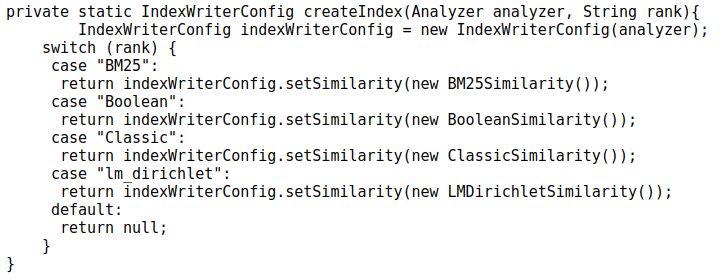
\includegraphics[scale=.35 ]{3} 
			\caption{Code Snippet of diffferent Scoring Similarities when Indexing}
			\label{fig:1}
		\end{center}
	\end{figure} \par



\section{Results}
Using trec\_eval I was able to get the results of each of the scoring methods. trec\_eval evaluates your results against a sample optimal results. \newline 


\begin{table}[H]
	\centering
	\begin{tabular}{|p{1.5cm}|p{1.25cm}|p{1.25cm}|p{1.25cm}|p{1.25cm}|}
	\hline Similarities & MAP & P30 & Recip. Rank & Recall \\ \hline
			BM25 					& 0.4067  & 0.1533 & 0.8262 & 0.8383 \\ \hline
			Classic 				& 0.3790  & 0.1481 & 0.7991 & 0.8148 \\ \hline
			lm\_dirichlet 			& 0.3096  & 0.1252 & 0.6958 & 0.7104 \\ \hline
			Boolean 				& 0.3006  & 0.1261 & 0.7072 & 0.7260 \\ \hline
			
	\end{tabular} 
	\caption{Results of each similarity lucence scoring}
	\label{table:results}
\end{table}
	
\newpage	
The BM25 similarity is the lucene scoring method that gives the best results and the boolean similarity is giving the worst results when evaluating against the optimal results.  BM25 is an improved version of Classic similarity as it uses a score for determining it will find a certain document relevant when scoring the documents. The boolean similarity gave the worst results as it only scores a document if it matches the query fully. This leaves gaps in the information retrieved. \par 

\section{Conclusion}
From creating a Search Engine in Lucene, I was able to gain a valuable insight into the information retrieval process in a larger scale. It allowed me to see the significant change in results when improving the analyser to allow for stop word removal and stemming  the words. Testing the different scoring methods was a great way to explore the Lucene libraries and methods.\par 

\section{Set Up}

\textbf{AWS Address}: \newline ec2-user@ec2-18-202-230-23
.eu-west-1.compute.amazonaws \newline .com \newline


\noindent \textbf{createIndex.jar}: creates an index of the cran collection, and stores in disk. To execute this file, run the following command:

\begin{center} 
 java -jar createIndex.jar \newline
\end{center}

\noindent \textbf{queryIndex.jar}: searches through the index, and returns results. The output results are stored in output directory. To execute this file, run the following command:

\begin{center} 
 java -jar queryIndex.jar \newline
\end{center}

\noindent \textbf{Results}: The files present in output directory, namely QRels.txt and results.txt can be used to evaluate metrics using TREC Eval tool. The command is as follows:

\begin{center} 
.. trec\_eval output/QRels.txt output/results.txt \newline
\end{center}

\noindent \textbf{To change the similarity method}: 

\noindent In the createIndex file replace the string input in this line of code to the preferred similarity:
	
\begin{center} 
	IndexWriterConfig config =  createIndex(analyzer, "enter here"); \newline
\end{center}

\noindent In the queryIndex file replace this line of code to the preferred similarity: 

\begin{center} 
	isearcher.setSimilarity(new BM25Similarity()); \newline
\end{center}

